\documentclass[11pt]{article}
\usepackage[utf8]{inputenc}
\usepackage{amsmath,amssymb}
\usepackage{graphicx}
\usepackage[backend=biber]{biblatex}
\addbibresource{example.bib}

\title{Approximating $s-t$ Minimum Cuts in $\Tilde{O}(n^2)$ Time Lecture Notes}
\author{Sourav Biswas, Quinlan Sykora}
\date{December 2022}

\begin{document}

\maketitle

\section{Problem Introduction}

We begin by introducing the concepts of cuts in graphs. Namely we define a cut $C$ to be defined as a partition of a graph into two groups. More formally, a cut $C$ is defined as two sets $V_1$ and $V_2$ such that 

\begin{equation}
    value(C) = \sum_{v_i \in V_1, v_j \in V_2} w_{ij}
\end{equation}

Assuming the weight between all vertices that don't have edges is zero. In general, cuts are useful concepts when dealing with graphs. Many problem have solutions that are ultimately derived from their minimum cut. For example, maximum flows across a graph are directly related to the minimum cut that separates our initial two nodes. Minimum bisection problems are similar equivalent to finding the minimum cut, and most relevantly, the conductivity of the graph, and therefore its second eigenvalue, is also directly related to the minimum cut in a graph.

\begin{equation}
    \frac{\nu_2}{2} \leq \Phi(G) \leq \sqrt{2 \nu_2}
\end{equation}

We furthermore observed in our first problem set how the diameter of the graph can be bounded by this conductivity. In summary, there are numerous uses of minimum cuts, and no truly flawless way to compute them.

\section{Definitions}

We will begin by defining some of the core concepts used in this work. 

\paragraph{K-connectivity}
Firstly, we will define the notion of K-connectivity. We define a graph to be k-connected if any cut that fully partitions the graph sever at least k edges. In the context of weighted graphs, we require that the total weight of the edges severed have a total weight of k or more. 

\begin{center}
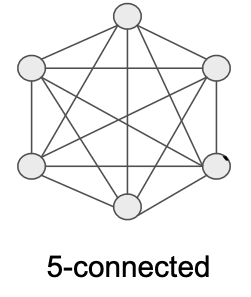
\includegraphics[width=0.2\textwidth]{figures/k_connected.png}
\end{center}

\paragraph{K-connected edge}
We extend the k-connectivity definition to individual edges in the graph. Namely, we say that an edge is k-connected if the minimum cut in the graph that includes that edge has a value of k. Essentially, the sparsest connection point that includes our given edge defines the k-connectivity of that edge.

\begin{center}
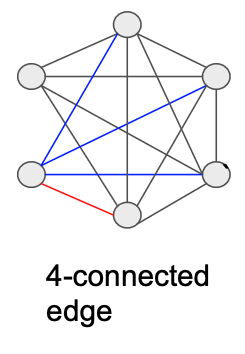
\includegraphics[width=0.2\textwidth]{figures/k_connected_edge.png}
\end{center}

\paragraph{K-strong component}
A K-strong component is defined as the maximal k-connected subgraph. This is essentially a group of k-connected vertices that are all k-connected to each other. The maximality means that we can't extend this cluster of points without including vertices that are not k-connected in the cluster. Note that the component can sometimes include the entire graph. 

\begin{center}
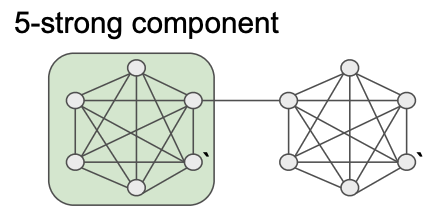
\includegraphics[width=0.5\textwidth]{figures/k_strong_component.png}
\end{center}

\paragraph{K-strong edge connectivity}
We define the K-strong edge connectivity (denoted as $c_e$) as the maximum value of k for which a strong component includes the given edge $e$. It can be intuitively thought of as the largest cluster that this particular edge is part of. 

\begin{center}
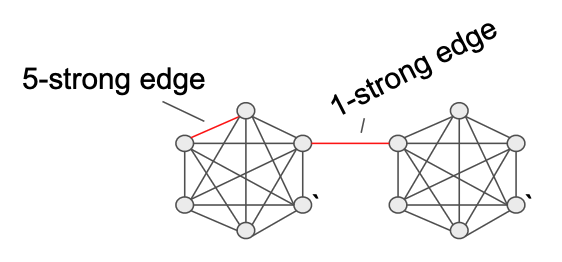
\includegraphics[width=0.5\textwidth]{figures/k_strong_edge_connectivity.png}
\end{center}

\paragraph{K-strong/K-weak edges}
An edge is called k-stong if it's k-strong edge connectivity $c_e$ is equal to or larger than k. Conversely, the edge is called k-weak if it's $c_e$ is less than or equal to k.

\section{Edge Sampling}

One of the first ideas that we have seen even in class is to randomly sample the edges. We showed previously that by changing the weight of the edges we can still have a high probability of approximating the minimum cut with an increasingly sparse graph. Let's begin by firstly sampling edges with the following probability:

\begin{equation}
    p = \Theta(\frac{log(n)}{\epsilon^2 c})
\end{equation}

Where $c$ is defined as the minimum cut in the graph. It has been proven in previous works \cite{Kar94a} that by sampling according to this probability, we can effectively approximate the cuts in a graph to within a factor of $\epsilon$

\begin{equation}
    \epsilon = \sqrt{2(d + 2)(\frac{M}{\hat{c}})ln(n)}
\end{equation}

With a corresponding probability of success of $1 - O(n^{-d})$. However, the main issue with this sampling theorem is that we are dependent on the minimum cut not being too small. We note that in this definition, the sampling theorem only works by setting each edge to be equal to a random variable with a maximum value of $M$ and sampling those random variables. For the edge case we can just make it equal to a Bernoulli distribution with a certain probability of being equal to 1. 

\begin{center}
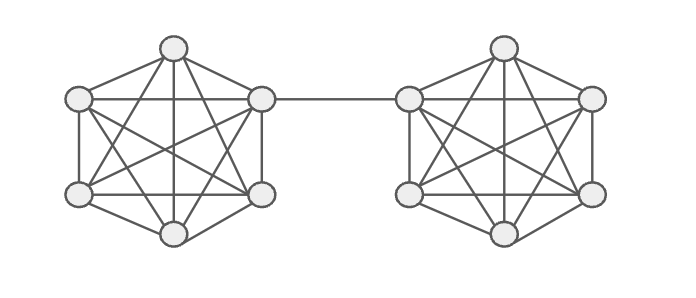
\includegraphics[width=0.8\textwidth]{figures/dumbell.png}
\end{center}

As seen in the figure above, the single edge connecting the two large clusters is effectively limiting the minimum probability that we can employ when sampling this graph. This is because the risk of that edge being sampled and prematurely cutting the graph would be too high otherwise. We therefore need a way to work around the sparsest regions of the graph when doing our sampling procedure. 

\section{Sparse Certificates}

Another important concept is a sparse certificate defined below:

\begin{center}
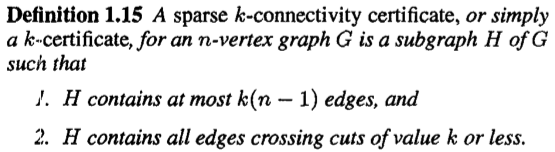
\includegraphics[width=0.8\textwidth]{figures/Def1_15.png}
\end{center}

\begin{center}
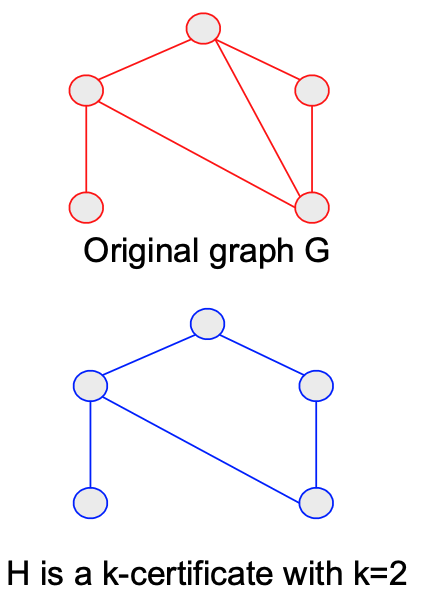
\includegraphics[width=0.3\textwidth]{figures/certificates.png}
\end{center}

High level idea: A graph $H$ with less edges than original graph $G$ and preserves cuts of value $\le k$. Therefore if we are interested in searching for cuts of value $\le k$ then its more efficient to look in $H$ instead of $G$ due to the reduced number of edges in $H$.

Recall Sampling Theorem 1.14 from earlier. We can combine sampling and sparse certificates in order to find cuts in graphs.

To find the minimum cut of value $c$ we can construct an $O(c)$ connectivity certificate which retains the same minimum cuts but reduces the edges in the graph to $O(nc)$. We can then use sampling with probability $\Theta((\log n)/c)$ to yield an $O(n\log n)$ edge graph with minimum cuts approximating the minimum cuts in the original graph. We can then use an algorithm to find minimum cuts noted in \cite{Gab95} to find min cuts in $\Tilde{O}(n)$ time (note this is ignoring logarithmic terms).

However to find an $s-t$ cut with value $v$ with a similar process involves sampling the $O(v)$ certificate of the original graph which reduces the edges to $\Tilde{O}(nv/c)$. Note we cannot use a sparser certificate without possibly damaging the cuts we are interested in finding. Similarly we cannot lower the sampling probability otherwise the variance of cut values will become too large. Therefore we become dependent on the ratio $v/c$. However, we can avoid this issue by using non-uniform sampling.

\section{Compression}

High level idea: Need compression to pay more attention to less dense areas and less attention to clustered areas. After compressing the graph - we can run existing algorithms for max flow, sparsest cut etc. 

\begin{center}
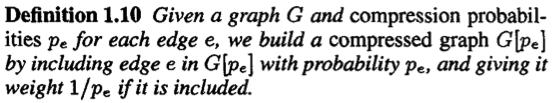
\includegraphics[width=0.8\textwidth]{figures/Def1_10.png}
\end{center}

Note that the expected value for each edge weight is 1 thus every cut has expected value after compression equal to its original value.

\begin{center}
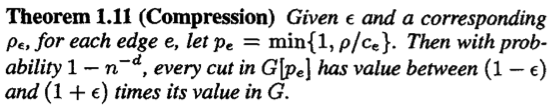
\includegraphics[width=0.8\textwidth]{figures/Thm1_11.png}
\end{center}

Theorem 1.11 notes we can compress the graph and keep cuts within constant bounds in the new graph.

\begin{center}
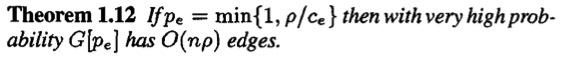
\includegraphics[width=0.8\textwidth]{figures/Thm1_12.png}
\end{center}

In the theorems a constant compression factor of $\rho_\epsilon = 16(d+2)(\ln n)/\epsilon^2$ is used for a given error bound $\epsilon$.

Theorem 1.12 allows us to use $\rho$ to get an approximation of $O(n\log n)$ for the number of edges in the compression graph. 

The proof for this theorem is essentially as follows. We will seek to produce an upper and a lower bound on the total number of edges produced using this sampling policy and find that that these bounds and exponentially convergent.

We begin with the idea of showing that graphs of a certain size must have a k-strong component. More specifically, we find that any graph of size $k(n-1)$ nodes must have at least one k-strong component. The proof for it is essentially a simple use of induction. 

We begin by finding the smallest graph with $k(n-1)$ nodes that does not have a k-strong component. You then take the nodes in the graph, find the smallest cut in the graph (which must be less than k) and determine that since this is the smallest graph without a k-strong component, it must have a value of less than k. We next determine that these two subgraphs created from the cut must also have less than $k(n'-1)$ nodes since otherwise they would contain the k-strong component. By adding together these components and counting up the edges, we find that we do not add back up to more than $k(n-1)$ edges, meaning there is not way of us having a graph of this size without it having a k-strong component.

\begin{center}
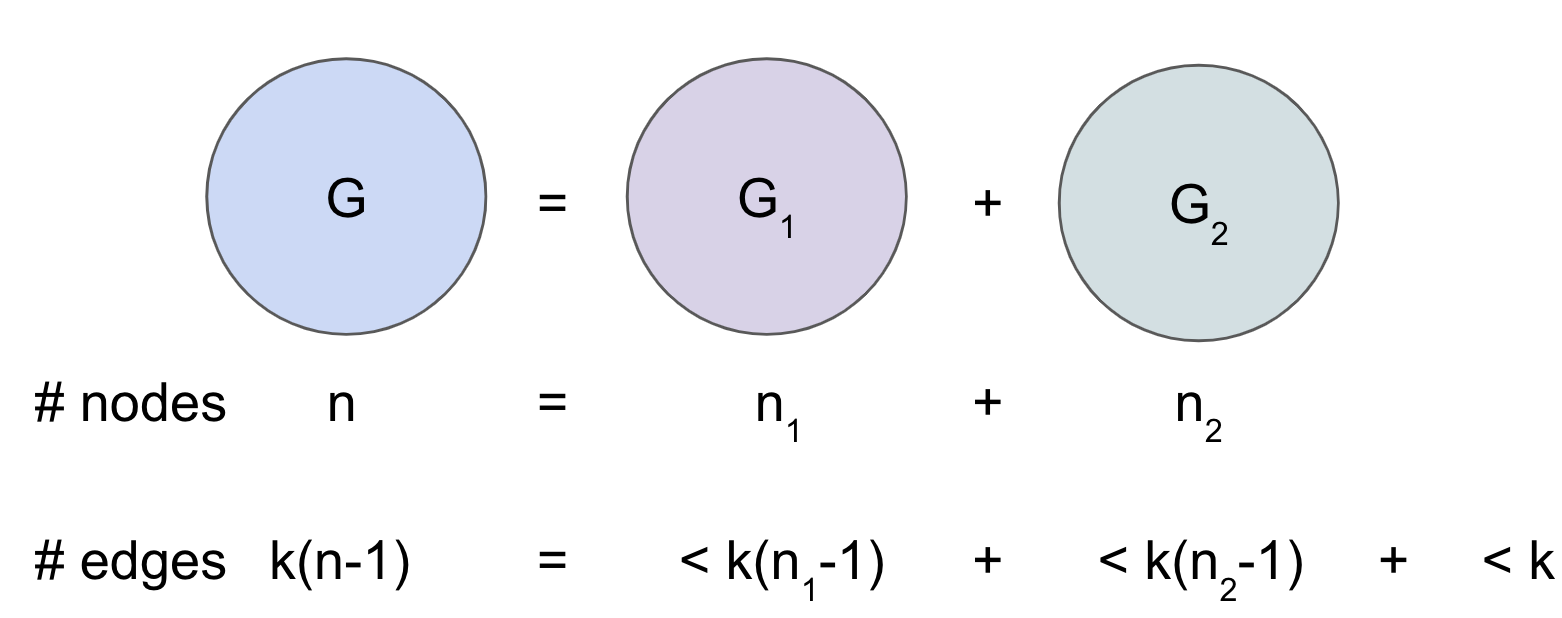
\includegraphics[width=0.8\textwidth]{figures/k_strong_lemma.png}
\end{center}

Now, we can return to our original formulation for the probability we use to sample each edge $p_e = min(1, \rho/c_e)$. Given this, we can create an inverse graph $G'$ where each edge is the inverse weight of the k-strong edge connectivity

can create an inverse graph $G'$ where each edge is the inverse weight of the k-strong edge connectivity.

\begin{equation}
    weight(e', G') = c_{e}^{-1}, \ \  \forall e' \in G
\end{equation}
 
We then can calculate the expected volume of the edges in the original graph relative to the weight of the edges in this new graph 

\begin{equation}
    \mathbb{E}[Vol(G[p_e])] = \sum_{e \in E} p_e \leq \rho \sum_{e \in E} c_e^{-1} = \rho \mathbb{E}[Vol(G'[p_e])]
\end{equation}

If this graph has a total edge weight of at most n, then this automatically gives is the total number of edges in the original graph by the above relation. We find that if the graph has more edges than n, then it must have a 1-strong component, and therefore must have a cut greater than 1. Let F be the component in the original graph that corresponds to this cut, and F' be the cut in the new graph G'. Given this fact, let $c_{e'}$ correspond to the minimum edge connectivity in this given cut.  We get from that that the value of the cut $VAL(C,F) \leq c_{e'}$, and also that since this is the 1 strong cut that $VAL(C,F') > 1$. However, we can also prove that 

\begin{center}
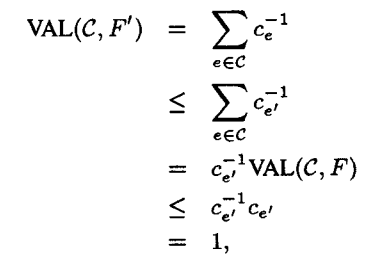
\includegraphics[width=0.4\textwidth]{figures/num_edges_proof.png}
\end{center}

Which is a contradiction and therefore there can't be a 1 strong component and the number of edges is bounded. 

\section{Error bounds}

The next step in this proof is going to be proving that the error bounds hold for this kind of sampling. The first thing that is proven is that we can generate an initial error bound of $O(\epsilon log(m))$ where $m$ is the total weights of all the edges in the graph. The way we will initially approach this problem is with subgraph edge sampling.

We will begin by sampling all edges that have a minimum cut that is less than 2.

\begin{equation}
    c_e \leq 2
\end{equation}

This creates the first sparsest subgraph. We then repeat the process of all edges that have strong weights between $2^1$ and $2^2$.

\begin{equation}
    2 \leq c_e \leq 4
\end{equation}

This can be repeated $log(m)$ times to encompass all edges in the graph. Each one of these groups we can effectively sample with a single probability to under-estimate the actual weight of each edge. Notice how each strong component is maintained in each of these graphs since we have all of the edges that make up each $c_e$ strong component. Therefore we can use the previous sampling theorem to evaluate the error on each subgraph. This results in us achieving the error bound $O(\epsilon log(m))$.

Now we will prove the better error bound. We will begin by defining $r_e^{(i)} = 2^{-(j-i)}$ where $j$ corresponds to the index of the power of 2 subgraph we are considering, namely $G_i$ which contains all edges where $2^i \leq c_e \leq 2^{i+1}$. We can then define a graph $H$ in such a way that for each edge we set it equal to a random variable 

\begin{center}
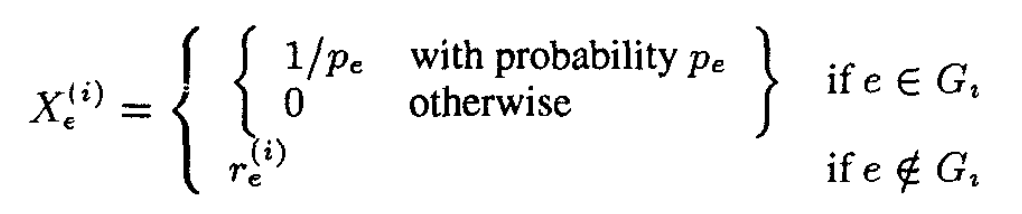
\includegraphics[width=0.8\textwidth]{figures/random_edge_variable.png}
\end{center}

Note that this is the same format as the sampling theorem random variables. The one difference from our above attempt, is we set the edges that aren't in this "phase" equal to a small value instead of being equal to 1.

Next, we need to show that the strength of this component $H$ of $G$ is maintained even with this reducing of the edge weight by a factor of $r_e^{(i)}$. We begin by defining $F_i$ to be the edges that have a strength of at least $2_i$. We can use induction to show that this holds.

\begin{center}
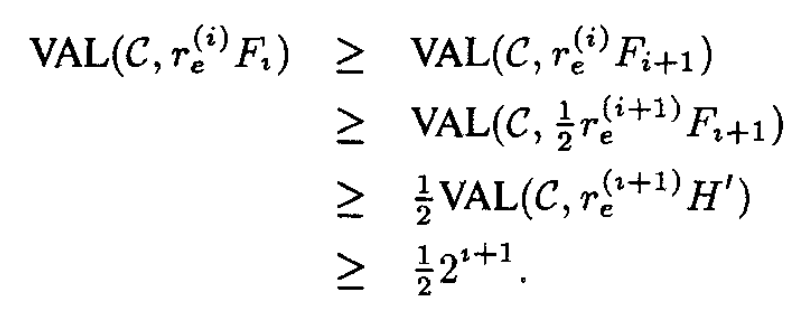
\includegraphics[width=0.8\textwidth]{figures/induction.png}
\end{center}

Where in this case we do reverse induction from the higher $F_{i+1}$ and where $H'$ is the $2^{i+1}$ strong component of this larger graph. 

Now, we can describe the previous sampled graph using these new subgraphs, since we can depict every phase as a subtraction between two of these subgraphs. More specifically, we can combine this with the original sampling theorem to get:

\begin{center}
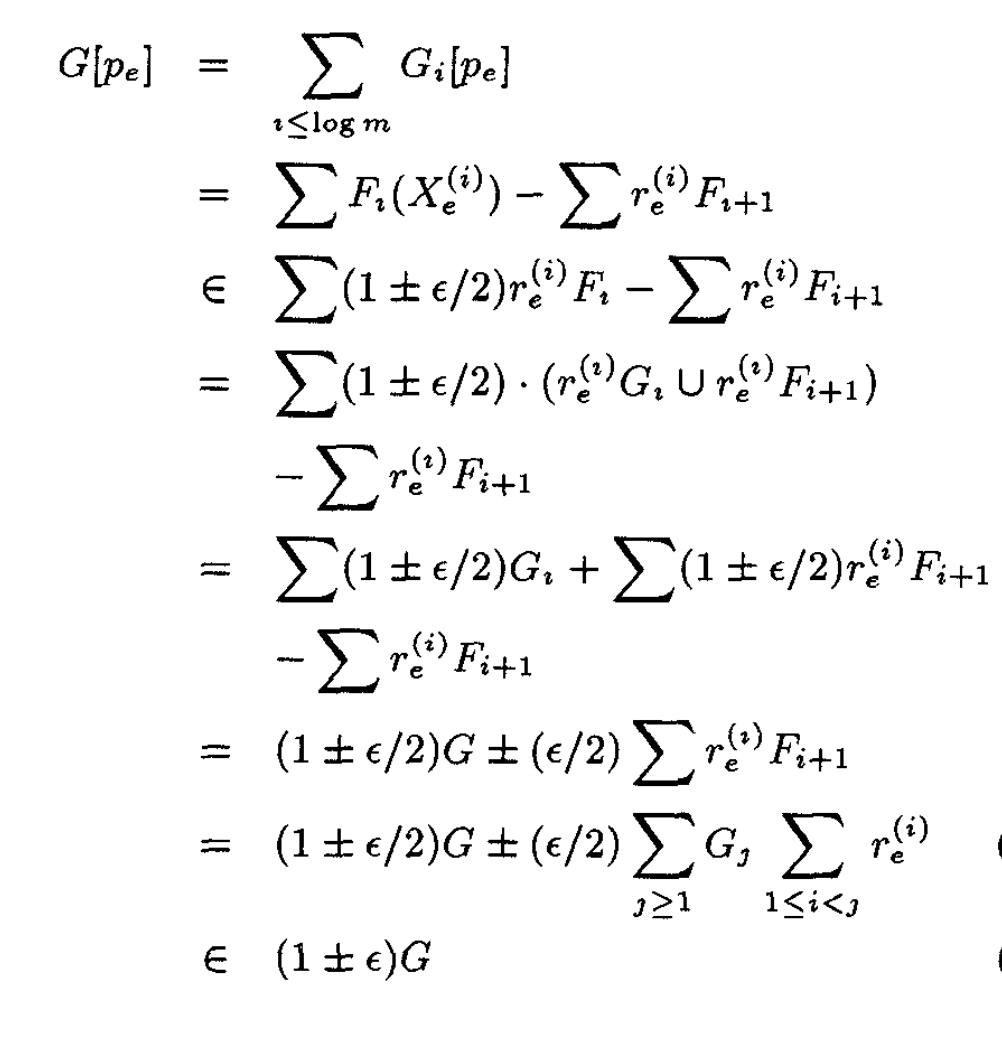
\includegraphics[width=0.4\textwidth]{figures/error_proof.png}
\end{center}

This therefore means that by looking at the sampling in a different way we can get the error bound we were originally loooking for.

\section{Finding Strong Connectivity}

So now that we know that this sampling method works, we need to find a way to determine the strong connectivity of the graph. Unfortunately, this problem is fundamentally NP hard, and therefore doesn't have a nice convenient solution. However, one way we could get around this is by using a polynomial time algorithm that allows us to lower bound the strong connectivity of a graph. We could use the previously mentioned algorithm for subdividing the graph, but this results in too many edges by a factor of $log(m)$ since we again have the recursive division of the graph.

Therefore, we first consider sampling for the k-weak edges in the graph. This will later on tell us which regions of the graph are the sparsest and to more or less avoid sampling. According to a previous work \cite{NI92b}, we can use the below algorithm to find these edges. This algorithm is able to run in $O(m log(n)$) time.

\begin{center}
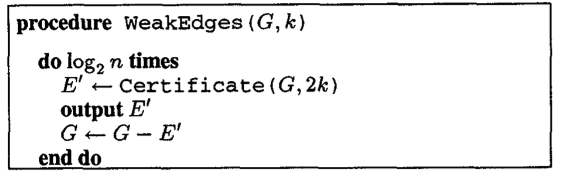
\includegraphics[width=0.8\textwidth]{figures/WeakEdges.png}
\end{center}

Given our above theorem on how many edges there are in k-weak graphs at most, we can find that this division into different graphs still results in $k(n-1)log(n)$ edges, which is again, not quite sparse enough for general purpose usage.

\section{Graph Partitioning}

One of the final proposed tools of this paper is to use a new algorithm called partition. This algorithm with output a new set of even sparser edges called the k-partition that we can use to produce the sparse graph. 

\begin{center}
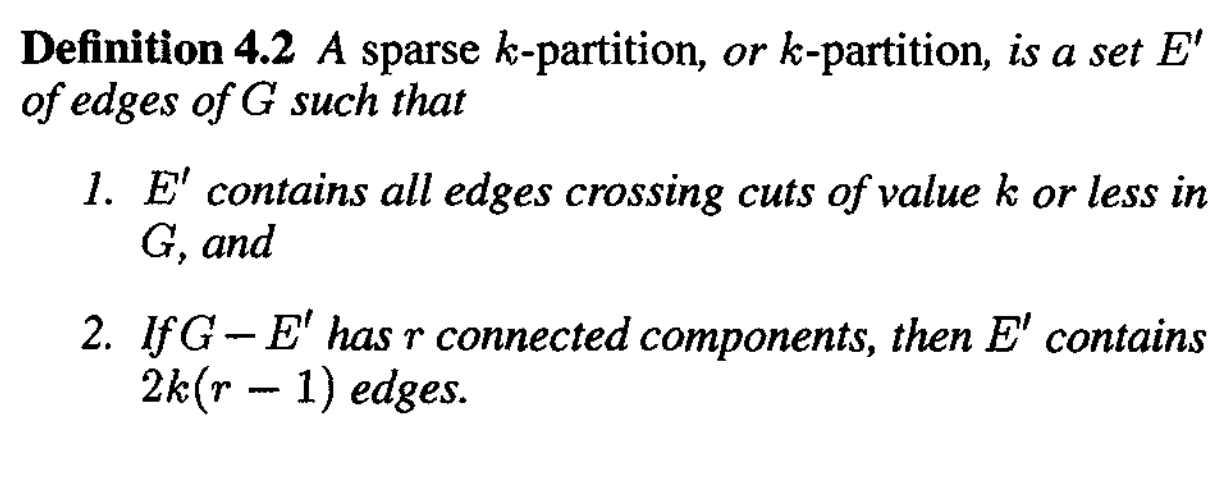
\includegraphics[width=0.8\textwidth]{figures/def_4_2.png}
\end{center}

We can derive such edge subsets by running the certificate algorithm seen above, and then replacing the edges that are still connected in the produced graph. When looking for the sparsest cuts, we can do this since these edges aren't actually cutting the graph and therefore aren't needed. This allows us to work with an even sparser subset of the edges in the graph itself. The algorithm can be seen below:

\begin{center}
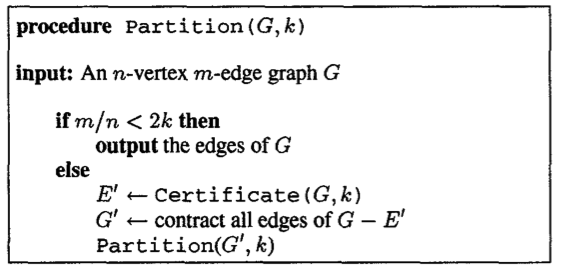
\includegraphics[width=0.8\textwidth]{figures/Partition.png}
\end{center}

The most important aspect of of this algorithm is that it finally allows us to operate without the dependency on the size of the graph in any way. Specifically, we find that the partition follows the following lemma:

\begin{center}
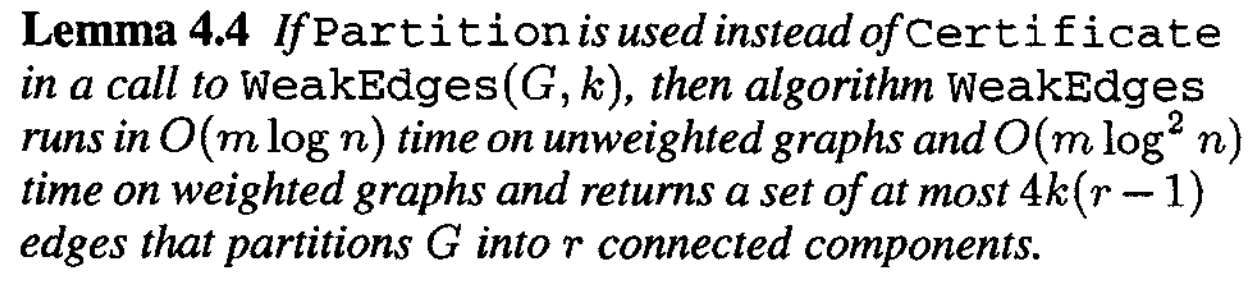
\includegraphics[width=0.8\textwidth]{figures/Lemma4_4.png}
\end{center}

Given this, we now know that we can produce the desired number of edges that allow us to compute cuts on a much sparser graphs. We can now consider all of the details together in the Estimation algorithm below.

Recall from earlier, if we have approximations $\Tilde{c_e}$ for the strong connectivities $c_e$ of edges in the graph then we could compress efficiently. The following algorithm allows us to find reasonably good lower bounds for the strong connectivities which we can then use for compression.

\begin{center}
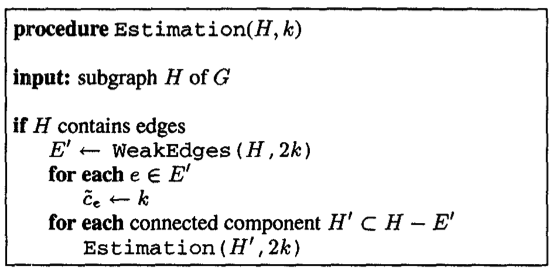
\includegraphics[width=0.8\textwidth]{figures/Estimation.png}
\end{center}

\begin{center}
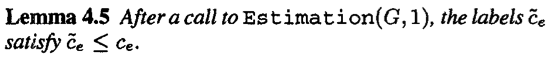
\includegraphics[width=0.8\textwidth]{figures/Lemma4_5.png}
\end{center}

From a high level, this algorithm recurses on components made of edges which are $2k$ strong in $H$ and thus are $2k$ strong in $G$. Therefore in the next level of recursion when we set $\Tilde{c_e} = 2k \le c_e$ for edges which are $4k$ weak then we know $\Tilde{c_e} = 2k \le c_e \le 4k$ which satisfies the lower bound we were aiming to achieve and noted in Lemma 4.5.

Thus with a call Estimation($G, 1$) we can estimate the strong connectivities in $G$.

\begin{center}
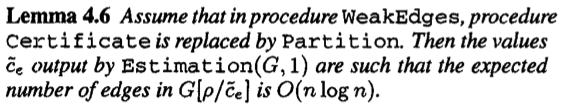
\includegraphics[width=0.8\textwidth]{figures/Lemma4_6.png}
\end{center}

Lemma 4.6 states that the compressed graph using these estimates for strong connectivity has $O(n\log n)$ edges.

We can prove Lemma 4.6 by induction and show that Estimation($G, k$) yields estimates $\Tilde{c_e}$ where $\sum{1/\Tilde{c_e}} \le 4(n-1)$. Showing this is sufficient since the number of edges then follows from Theorem 1.12. 

Aside from the trivial base case of one vertex, we consider the induction case with Estimation($G, k$). WeakEdges returns $4k(r-1)$ edges that split $G$ into $r$ components $G_1, ... , G_r$. Suppose these components have sizes $n_1, ..., n_r$ and WLOG $r > 1$. Note the recursive calls to Estimation on each $G_i$ implies by induction we have strong connectivity estimates $\Tilde{c_e}$ for each $G_i$ where $\sum_{e \in G_i}{1/\Tilde{c_e}} \le 4(n_i - 1)$. 

Note for the $4k(r-1)$ edges not in the components $G_i$ we assign their estimates $\Tilde{c_e} = k$ yielding: 

\[
\sum_e{1/\Tilde{c_e}} \le \sum_i{4(n_i - 1)} + \sum_{e \notin G_i}{1/k}
\]

\[
\le \sum_i{4(n_i - 1)} + 4k(r-1)/k
\]

\[
\le 4\sum_i{n_i} - 4r + 4(r-1)
\]

\[
\le 4(n-1)
\]

\begin{center}
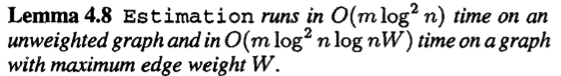
\includegraphics[width=0.8\textwidth]{figures/Lemma4_8.png}
\end{center}

The runtime in Lemma 4.8 is found by noting WeakEdges is called $m$ times with a maximum $O(\log m)$ recursions since the max strong connectivity is $m$. Similarly for weighted graphs the maximum recursions is $O(\log nW)$ where $W$ is the maximum edge weight. 

\section{Modifications for Weighted Graphs}

To extend the approach to weighted graphs, a few modifications are needed. The main theorems 1.11 and 1.12 still hold for weighted graphs if weights are scaled up, rounded to integers, and edges of weight $w$ are replaced with $w$ copies of the same edge. 

However note that the runtimes for the algorithms become unreasonable with the potentially large number of duplicated edges. 

\begin{center}
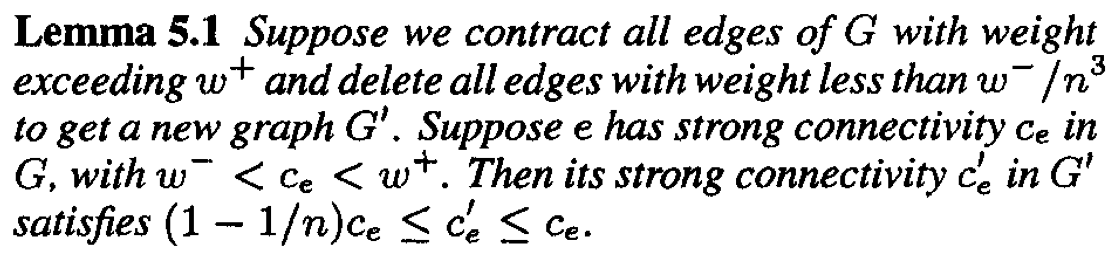
\includegraphics[width=0.8\textwidth]{figures/Lemma5_1.png}
\end{center}

The intuition behind Lemma 5.1 is instead of considering the entire weighted graph, we can limit our focus to edges within a certain range and the strong connectivities in this graph approximate the strong connectivities in the original graph reasonably well.

To prove Lemma 5.1 we can first prove $c_e' \le c_e$. Proceed by contradiction and suppose after contracting we have an edge $e$ in component $H'$ with $c_e' > c_e$. Now consider the original component $H$ in $G$ which must have connectivity $ \le c_e$. Since $H'$ was obtained by contracting all edges of weight over $w^+$ from $H$, then there is a cut with value $c_e < w^+$. Based on how $H'$ is generated only removing edges with weights over $w^+$ then no edge across the cut in $H$ is removed so it still has value $c_e$ in $H'$ which is a contradiction.

On the other hand, we can see the total weight of removed edges is 

$\le {n \choose 2} w^- / n^3 < c_e/n$ 
which proves the lower bound $c_e' > c_e(1 - 1/n)$.

\begin{center}
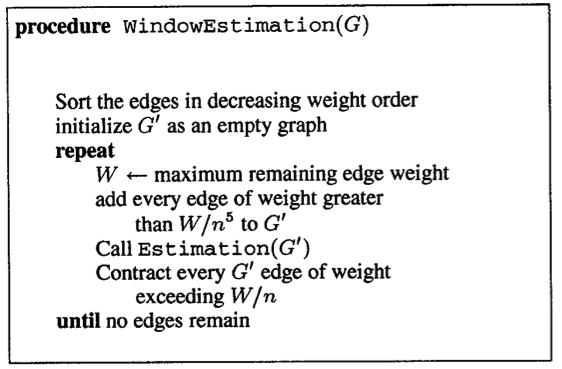
\includegraphics[width=0.8\textwidth]{figures/WindowEstimation.png}
\end{center}

We can then modify the Estimation algorithm to only focus within windows of relevant connectivity and call the previous Estimation algorithm within each window. Note that we can use a union-find data structure for adding and contracting edges. Since the window range is $W/n^5$ to $W$, each edge is in the window a maximum of 5 times. Therefore the total size of graphs passed to Estimation is $O(m)$. Therefore the runtime of WindowEstimation is $O(m\log^2 n)$

\begin{center}
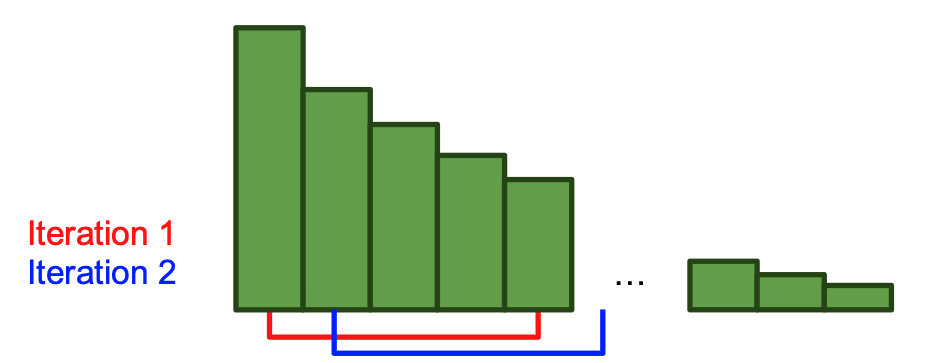
\includegraphics[width=0.8\textwidth]{figures/window.png}
\end{center}



\section{Applications}

We can use the simplified compressed graph $G[p_e]$ with reduced edges along with existing algorithms to reduce the overall runtimes for different applications.

\subsection{$s-t$ Min Cut}

Note that minimum cut values are approximated in the compressed graph denoted by $VAL(C, G[p_e]) \le (1+\epsilon)v$. We also know that the compressed graph has $O(n\log n / \epsilon^2)$ edges. Therefore we can use a maximum flow algorithm \cite{GT88} on the compressed graph $G[p_e]$ to find the minimum $s-t$ cut in $O(n^2\log^2 n / \epsilon^2)$ time.

\subsection{Sparsest Cut}

To find the sparsest cut we are looking for the cut that minimizes the ratio: 

\begin{center}
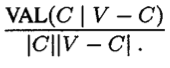
\includegraphics[width=0.2\textwidth]{figures/SparsestCut.png}
\end{center}

Similar to before, we can use an existing algorithm \cite{KST90} to find the sparsest cut $O(\log n)$ approximation in $O(m^2 \log m)$ time. Therefore by running this algorithm on the compressed graph we can find a similar $O(\log n)$ approximation but instead in $O(n^2 \log^3 n / \epsilon^4)$ time.


\section{Future Steps}

Compression is relying heavily on simplified versions of the original graph which approximate the values of cuts in the original graph. One future direction is to try and make these approximations exact. There are existing works \cite{Kar96} which have exact linear time solutions however this appears to only be for specific problems and will not work in the general case.


\printbibliography

\end{document}
https://www.overleaf.com/project/637ed0ddee248caf7675e974

